\documentclass{llncs}
\newcommand{\Section}[1]{\vspace{-8pt}\section{\hskip-1em.~~#1}\vspace{-3pt}}
\newcommand{\SubSection}[1]{\vspace{-3pt}\subsection{\hskip -1em.~~#1}\vspace{-3pt}}
\newcommand{\X}{{\bf X}}
\newcommand{\x}{{\bf x}}
\newcommand{\Y}{{\bf Y}}
\newcommand{\y}{{\bf y}}
\newcommand{\Z}{{\bf Z}}
\newcommand{\z}{{\bf z}}
\newcommand{\bs}{\boldsymbol}
\newcommand{\bSigma}{\boldsymbol \Sigma}
\usepackage{amsmath,amssymb,algorithm,algorithmic}
\usepackage{times}
\usepackage{setspace,verbatim}
\usepackage{epsfig,url}
\newcommand{\argmax}{\operatornamewithlimits{argmax}}


\begin{document}
\vspace{-0.1in}
\title{Anatomically-Constrained PCA for Image Parcellation}
\author{Anonymous}
\institute{Anonymous}
\maketitle              
%\vspace{-0.1in}
\begin{abstract}
 Traditionally clinicians and medical researchers have been using either totally data driven approaches like PCA/CCA/ICA or ROI based analysis for exploratory analysis of brain images. However, PCA/CCA/ICA based approaches suffer from lack of interpretability of results and on the other hand ROI based approaches are too rigid and wrongly assume that the signal lies totally within a predefined region. In this paper, we propose a novel approach which stands in stark contrast with both these approaches as it borrows strength from both these paradigms and leads to refined definitions of ROIs based on information from data. Our approach, called Prior Constrained PCA (AC-PCA) provides a principled way of incorporating prior information in the form of ROIs while still allowing the data to softly modify the original ROI definitions. Experimental results on cortical thickness images show the superiority of AC-PCA for MCI classification compared to ROI and unconstrained PCA (a totally data based approach). 

\end{abstract}

\section{Introduction and Related Work}
Over the last  few decades there have been significant breakthroughs in medical imaging machinery which has led to an increase in the amount and diversity of data being available e.g. structural and functional modalities, neurocognitive batteries, genetics, and environmental measurements etc. This has lead to a substantial interest in using sophisticated statistical methods to analyze and explore this data. Methods like Principal Component Analysis (PCA), Independent Component Analysis (ICA), Canonical Correlation Analysis (CCA) and their robust and sparse variants have been the workhorse of brain and neuro imaging fields as they provide key insights into the data in a totally data driven way. Particularly they find directions of maximum variance in data or its close variant and show the signal to lie in a small number of succinct regions in brain. 

However, one potential pitfall of these approaches, which has made clinicians and other researchers cautious with their use is the lack of control over the areas they highlight. Since, they work in a totally data driven way the end clinician/researcher has little control over the areas of brain they chose. Clinicians usually have some form of prior knowledge as to which areas may contain the signal they are looking for, for example, someone studying fronto-temporal dementia would expect some or most of the signal to lie in frontal cortex, however if the voxels in frontal cortex don't explain the variance in data these approaches won't highlight them. 


So, this has led the clinicians and researchers to work with totally prior driven approaches e.g. ROI (Region of Interest) analysis, where they chose a pre-defined region manually or based on past study (for instance {\em Brodmann Areas}) and study it exclusively. In other words, they wrongly assume that the entire signal is confined with in that region, i.e. frontal cortex in the above example. Though, it is not a terrible assumption that the signal lies entirely in that confined region however they are missing some important signal from data. Also, the label set might not generalize across population and different datasets as there is lots of variation in people and {\it Brodmann's} definitions might not provide the most general sets of labels. 
When effects are localized to the selected region, and that region is well-defined, an ROI analysis may
provide the most sensitive testing method.  However, some conditions
involve a network of regions that may not be fully identified.
Furthermore, effects may not localize to the boundaries of a
classically defined ROI.  In such cases---in addition to the general
case of an exploratory analysis in a small dataset---dimensionality
reduction may provide advantages over an ROI analysis or mass
univariate voxel-based morphometry \cite{Ashburner2005}.

\begin{figure*}
\begin{center}
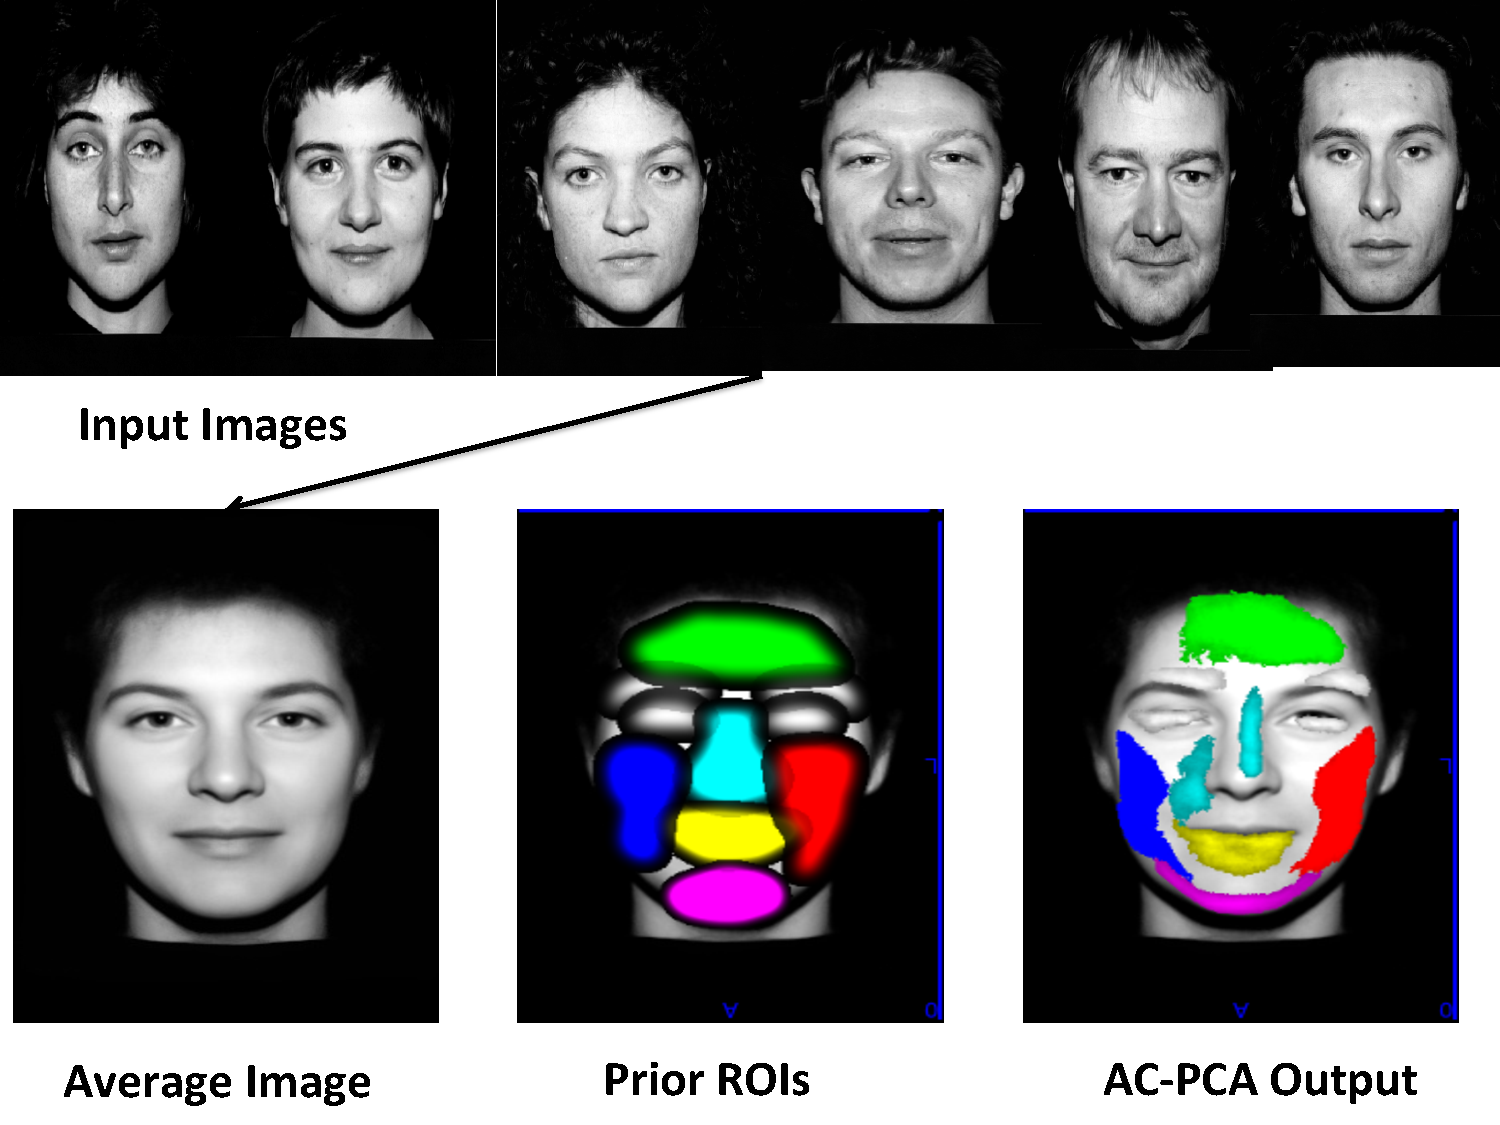
\includegraphics[width=0.7\linewidth]{fig1.pdf} 
\end{center}
\vspace{-0.2in}
\caption{AC-PCA pipeline: 1) Take in raw images 2). Register them and create an average image 3). Define Prior ROIs 4). Run (AC-PCA) which weighs both data and prior ROIs }
\label{fig:faces}
\end{figure*}



In this paper we propose an approach which addresses the weaknesses of both the methodologies described above, particularly, the lack of interpretability for statistical methods and wrong assumption of hard label boundaries for ROI based analysis. Our approach, called Anatomically Constrained PCA (AC-PCA),  takes into account the neuro-anatomical variation in people while creating the ROI labels. This allows us to modify the definitions of labels to capture the variation in dataset while still staying close to the initial ROI definitions. AC-PCA provides probabilistic labels with ``soft'' boundaries and as we show in the experimental section, these ``soft'' boundaries are more sensitive to the activity in brain.

Our approach provides a principled way of incorporating priors in a totally data driven approach based on PCA. Our optimization objective provides a tradeoff between 1). staying close to the initial ROI definitions and 2). allowing data to lead the exploratory analysis by explaining variance through PCA. A good way to think about this is as ROI definitions forcing us to be {\em conservative} and staying close to the initial definitions e.g. {\it Brodmann's} areas; on the other hand the PCA component gives us {\em liberty} to be more exploratory and just trust the given data. The tradeoff between the two competing paradigms is defined by user tunable parameter, which is chosen via cross validation on a separately held validation set. Figure~\ref{fig:faces} gives an example of proof of concept of our approach using faces and also explain our general experimental pipeline used throughout this paper.


The remaining paper is organized as follows; in next section we provide the details of AC-PCA and provide an algorithm which implements our approach. In Section 3, we provide experimental results on synthetic and real datasets showing the efficacy of our approach and its superiority to both the alternatives mentioned above.


\section{ Anatomicallly Constrained Principal Component Analysis: AC-PCA}
Lets assume that we are given a data matrix ${\bf X}$ where each row represents a patient (total {\bf n} of them) and each column represents a voxel in image (total {\bf p} of them). In practice, we usually have ${\bf p \gg n}$. Also, lets assume that we have a prior matrix {$\bf M(\lambda)$} (function of a parameter $lambda$ which controls its strength) whose each row corresponds to a separate prior e.g. different Brodmann areas (total {\bf k} of them) and each column (total {\bf p} of them) contains the probability of a particular voxel belonging to that prior.  

A totally data driven approach like vanilla PCA would ignore the prior matrix {\bf M} completely and just try to find combinations of voxels that explain the most variance. The objective it optimizes is:

\begin{equation}
{\bf v_i^*}= \argmax_{{\bf v_i},{\bf \|v_i\|}=1} {\bf v_i}^{\top}{\bf X^{\top}X}{\bf v_i}
\label{pca}
\end{equation}
where {$\bf v_i^*$} is the $i^{th}$ the direction of maximum variance (called eigenvector) of data matrix {\bf X}. These vectors when plotted on the image highlight regions of image which PCA (i.e. a totally data driven approach) thinks are relevant. Since, we have ${\bf p \gg n}$, the above is an ill-posed problem and we need sparsity in eigenvectors, which gives rise to Sparse PCA. The objective is exactly the same as Equation~\ref{pca} except that now we have an additional sparsity penalty ($\|\bf v \|_1$) on eigenvectors.


Our proposed algorithm AC-PCA builds on Equation~\ref{pca} and adds an additional term to the objective for incorporating prior information. Basically, it says that instead of finding the eigenvectors of the data covariance matrix (as a totally data driven approach would do), find the eigenvectors of the transformed data covariance matrix obtained by projecting it to the prior space. An important consequence of this is that we are not confining our data driven priors to lie in the original ROIs rather we are encouraging them to find ways to explain data variance but in this new ``prior projected'' space.  Also, note that instead of taking the prior as is, we smooth it as $M^s_i=\exp(\frac{M_i-1}{\lambda})$ before using it in our optimization. The modified objective is given below:
\begin{equation}
\label{ppca}
{\bf v_i^*}= \argmax_{{\bf v_i},{\bf \|v_i\|}=1} {\bf v_i}^{\top}{\bf diag(M^s_i(\lambda))}{\bf C}{\bf v_i} - \eta\cdot\|\bf v_i \|_1
\end{equation}
where ${\bf M^s_i(\lambda)}$ is  the ``smoothed'' the prior corresponding to the $i^{th}$ eigenvector and is itself a vector of size (${\bf 1\times p}$) and $\bf C$ is the data covariance matrix ($\bf X^{\top}X$). The {\bf diag} operator converts the ${\bf 1\times p}$ vector into a ${\bf p\times p}$ matrix and is used just for notational convenience.  $\lambda$ is a user tunable parameter which controls the tradeoff between the influence of data and prior and should be typically tuned on a held out validation set. Its easy to see that smaller values of $\lambda$ suggest that we trust prior more and as $\lambda$ is increased we want our eigenvectors {\bf v} to be influenced more and more by the data. Also, it is important to note that we set the sparsity parameter $\eta$ automatically as $\frac{Number\;\;of\;\;voxels\;\;in\;\;Prior\;\;ROI}{Total\;\;Number\;\;of\;\;Voxels\;\;in\;\;Brain}$. 

Figure~\ref{fig:priorvary} shows the effect of varying the $\lambda$ parameter on the $(PC)^2A$ performance. As mentioned earlier, we choose $\lambda$ by cross-validation on a validation set.

\begin{figure*}
\begin{center}
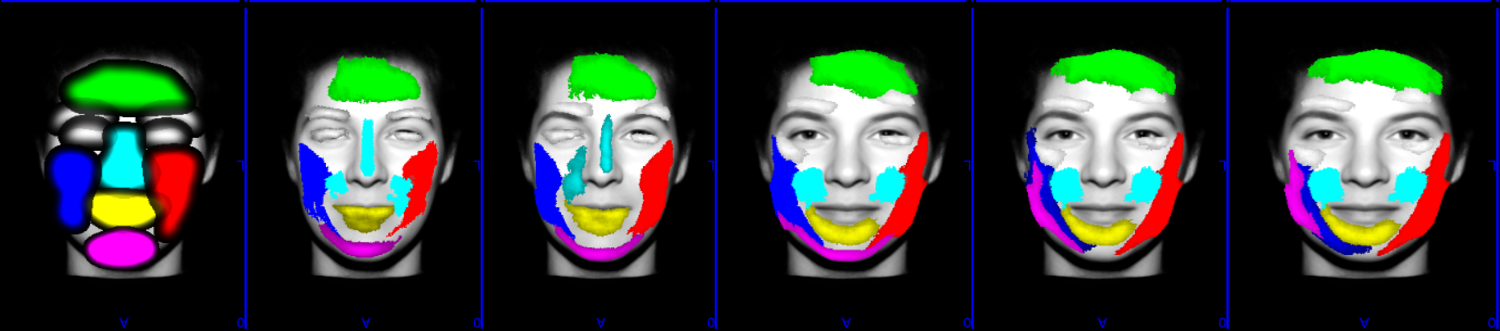
\includegraphics[width=\linewidth]{fig2.pdf} 
\end{center}
\vspace{-0.2in}
\caption{(AC-PCA) outputs for $\lambda=[0.0,0.2,0.5,2.0,5.0,10.0]$ from left to right. Note that $\lambda =0$ corresponds to using only prior ROIs and as $\lambda$ is increased effect of data increases. This is evident from the fact that with increasing $\lambda$ our priors especially around {\em nose, eyes and eyebrows} are getting washed away.}
\label{fig:priorvary}
\end{figure*}



\subsection{An Algorithm for AC-PCA}
Since our data matrices are huge, typical number of voxels in image ${\bf p}\approx 100000$, simple methods which use routines from R, MATLAB don't scale that well. Instead, we propose a fast and novel iterative algorithm in C++ (publicly available) for solving the above optimization problem. The algorithm is presented below in Algorithm~\ref{algo1}.


\begin{algorithm}[htdp]
\small \caption{\bf Prior Constrained Principal Component Analysis: AC-PCA}
\label{algo1}
\begin{algorithmic}[1]
\STATE Normalize the data matrix {\bf X} by  mean centering it.
\STATE Select the (fractional) sparsity parameter $\eta$ and prior scale parameter $\lambda$
\STATE Uniformly initialize the $k$ eigenvectors $\bs v_{1,\ldots, k} \gets 1/p$ and set $j=0$.

\WHILE {$\|{\bf v_{1,\ldots,k}^{j+1}-v_{1,\ldots,k}^{j}}\|$) $<$ $\epsilon$}
\FOR {i=1 to k}
\STATE ${\bf v_i^{j}}$ $\gets$ ${\bf Xv_i^{j-1}}$ //Implements modified Arnoldi Iteration algorithm
\STATE ${\bf v_i^{j}}$ $\gets$ ${\bf X^{\top}v_i^{j}}$
\STATE ${\bf v_i^{j}}$ $\gets$ ${\bf v_i^{j}}\cdot \bf M^s_i$ // Update the eigenvector estimate with prior information.
\STATE Orthogonalize the eigenvector with respect to all other eigenvectors:\\ ${\bf v_i^{j}} \gets {\bf v_i^{j}} - \sum_{l <i} \frac{\bf v_i^{j} \bf v_l^{j}}{\bf v_l^{j} \bf v_l^{j}}  \bf v_l^{j}$
\STATE Soft-Max Sparseness:  ${\bf v_i^{j}}  \leftarrow (\|{\bf v_i^{j}}\|  - max({\bf v_i^{j}})*\eta)_+ Sign({\bf v_i^{j}})$ //Note that $\eta$ is set automatically as described earlier.
%\STATE Cluster Threhold: 
\STATE Normalize the eigenvector ${\bf v_i^{j}}$ $\gets$ ${\bf v_i^{j}}/\|{\bf v_i^{j}}\|$
\ENDFOR
\STATE j $\leftarrow$ j+1
\ENDWHILE
\end{algorithmic}
\end{algorithm}


\section{Experimental Results}
In this section we show the performance of our approach on cortical thickness images. Our data consists of images from 222 individuals, of whom 111 were diagnosed clinically with Mild Cognitive Impairment (MCI) and the remaining 111 were normal age matched controls. %add info. about age and gender
All images were acquired with a Siemens Trio 3.0 Tesla MRI scanner. The analysis of T1 images was done using publicly available Advanced Normalization Tools (ANTS, \url{http://www.picsl.upenn.edu/ANTS/}) and the associated pipelining framework PipeDream ({\url{http://sourceforge.net/projects/neuropipedream/}) which mapped each subject to an existing, elderly/neurodegenerative population template, built from images acquired from the same scanner and imaging parameters.

We used two cortical label definitions for our experiments 1). Non-Rigid Image Registration Evaluation Project (NIREP), \url{http://www.nirep.org/}, 32 labels in total and  2). LONI Probabilistic Brain Atlas (LPBA40)~\cite{lpba} 55 labels in total.


We ran (AC-PCA) independently for each label set with varying values of prior strengths, $\lambda =[0.1,0.2,0.5,1.0,2.0,5.0,10.0,20.0]$.

\begin{figure*}
\begin{center}
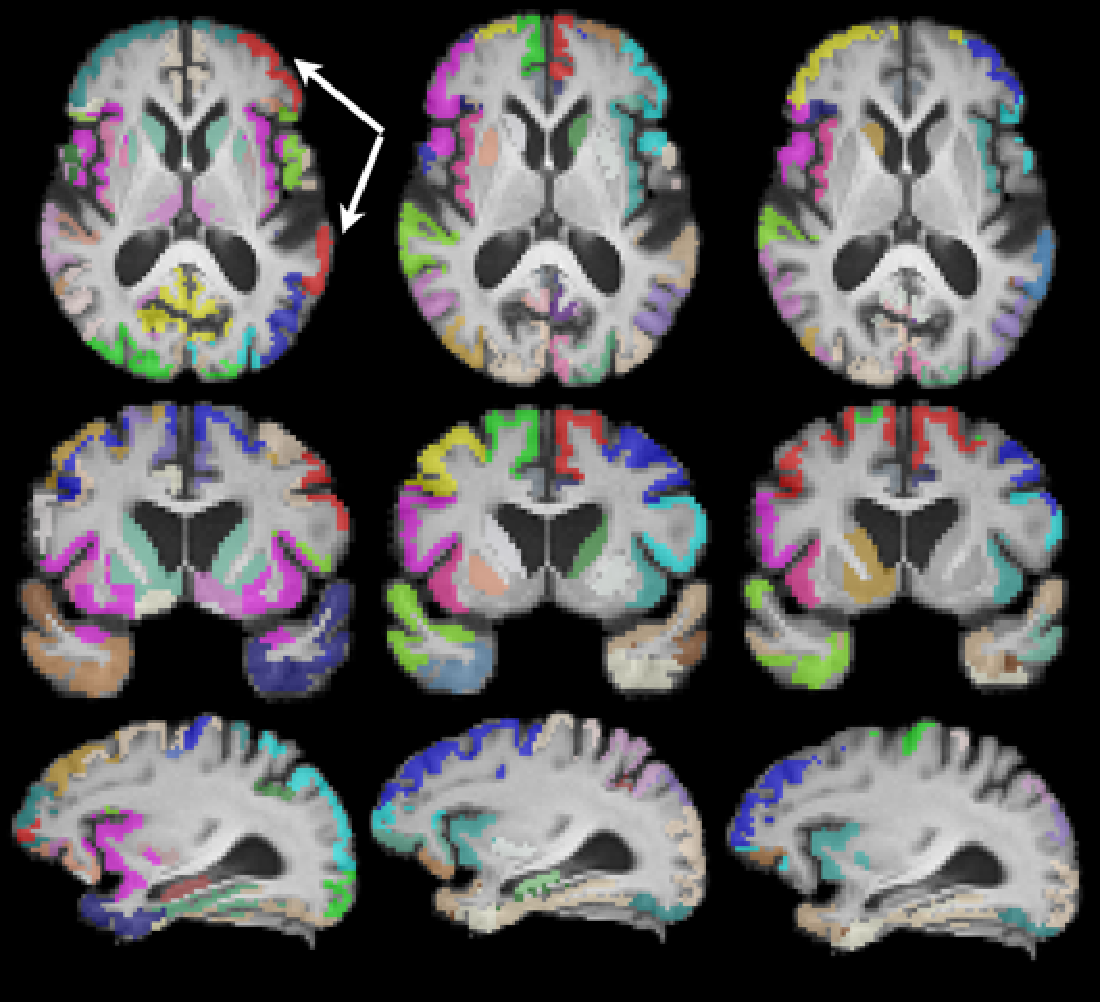
\includegraphics[width=0.8\linewidth]{lpba.pdf} 
\end{center}
\vspace{-0.2in}
\caption{Results for LPBA40 labels. Left to right- Unconstrained PCA, prior LPBA labels, AC-PCA labels. The arrows show left frontal gyrus and the left superior temporal gyrus.}
\label{fig:priorlpba}
\end{figure*}


\subsection{Qualitative Results}

The figures below show slices of axial and sagittal section labelings for unconstrained PCA, true cortical labels (NIREP and LPBA40) and prior constrained PCA (AC-PCA).

% As can be seen from the figures, the prior constrained labelings have been modified from their prior anatomical definitions (i.e. NIREP or LPBA) based on evidence from data. However, unlike unconstrained PCA, the AC-PCA labels are more spatially constrained and do not generate the same label for distant but correlated brain structures. 
%As can be seen from the figures, there is a one-one correspondence between prior anatomical labels and the labeling generated by AC-PCA as we have constrained them to stay near to their prior labels, however such a correspondence does not exist between the labels generated by unconstrained PCA and prior labels  

In the unconstrained PCA, the same label is assigned to parts of the left frontal gyrus and the left superior temporal gyrus (shown by arrows in figure) since it has no notion of anatomy; on the other hand, AC-PCA, since it is anatomical prior driven does not join distant structures which aids interpretability.

Another interesting observation is that both AC-PCA and unconstrained PCA have assigned  the same label to corresponding regions in the left and right hemispheres. This occurs less frequently in AC-PCA as we have constrained it via anatomical priors.  %The anatomical constraint is less effective for structures close to the mid-line of the brain because these structures are closer to the corresponding structure on the other hemisphere.
%%since based on euclidean distance structures on opposite hemispheres which are close to each other can have same label.

\begin{figure*}
\begin{center}
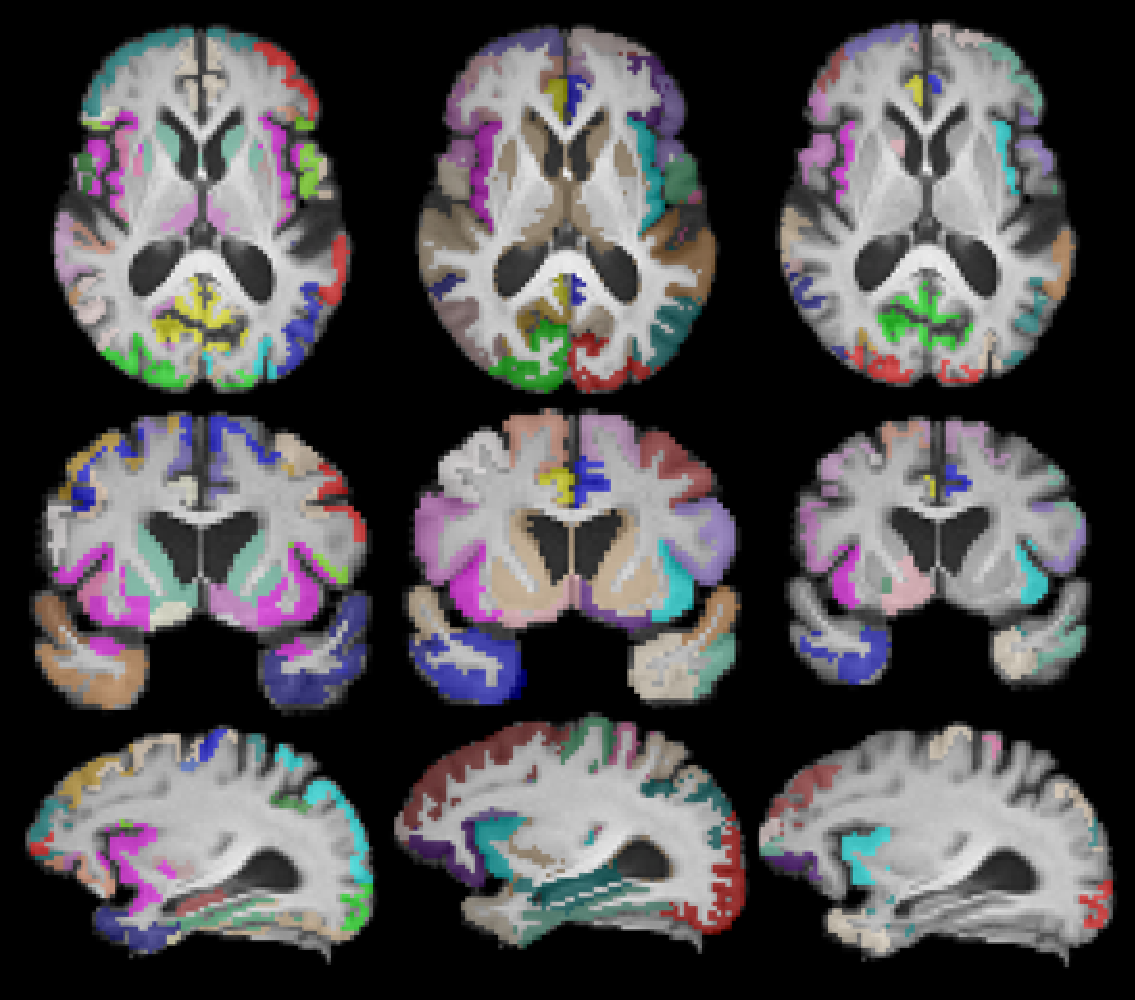
\includegraphics[width=0.8\linewidth]{nirep.pdf} 
\end{center}
\vspace{-0.2in}
\caption{Results for NIREP labels. Left to right- Unconstrained PCA, prior NIREP labels, AC-PCA labels}
\label{fig:priornirep}
\end{figure*}



\subsection{Classification of MCI vs Normal}
We use the projections (eigenvectors projected onto the data matrix) resulting from unconstrained PCA, AC-PCA and prior cortical labels to distinguish individuals with Mild Cognitive Impairment (MCI) from normal aging individuals. 
Since it is a classification problem, we used logistic regression and randomly split the data into training ($80\%$), validation ($10\%$) and testing ($10\%$). Firstly, we use cross validation to determine the best value of prior strength parameter ($\lambda$); we train on the training data and test on validation data with varying prior strengths as mentioned above and then choose the best value of prior strength as the one which gave the least classification error on the validation set.  The best prior strength value was $\lambda =0.5$ for NIREP labels and $\lambda=0.2$ for LPBA40 labels. 

Next, with these values of $\lambda$ we trained AC-PCA on the entire training and validation set and tested on the test set. This whole procedure was repeated 10000 times and the classification accuracies are given in Table 1.

As can be seen from the table, the AC-PCA significantly (paired t-test) outperforms unconstrained PCA as well as the approach which just uses cortical ROI labels hence leading to a classifier which can better distinguish MCI patients from normal controls. 


\begin{table}
\begin{center}
\begin{small}
\begin{tabular}{|c|c|c|c|}
\hline
 Label Set& Unconstrained PCA ($\mu\pm\sigma$) & ROI Cortical Labels ($\mu\pm\sigma$) & AC-PCA ($\mu\pm\sigma$)  \\
\hline
 NIREP& $62.58\% \pm 4.5\%$&$66.05\pm 3.9\%$ &${\bf 67.96\%\pm 2.3\%}$\\
 LPBA40&$62.58\% \pm 4.5\%$&$65.95\%\pm3.6\%$ &${\bf 67.15\%\pm 3.2\%}$\\ 
   \hline
\end{tabular}
\end{small}
\vspace{0.1in}
\caption{Test Set classification accuracies averaged over 10000 runs (More details in text). AC-PCA is significantly ($p-val <0.0001$ in paired t-test) better than Unconstrained PCA and ROI Cortical Labels}
\end{center}
\end{table}


\section{Conclusion}
In this paper we proposed a novel approach for incorporating prior information in the form of anatomical priors into totally data driven approaches like PCA. We augmented the basic PCA objective to take into account prior anatomical information and proposed a fast modified Arnoldi iteration algorithm to solve the optimization problem. 
We also illustrated the benefits of our approach over standard unconstrained PCA as well as ROI based analysis by experiments on cortical thickness images which shows the superiority of AC-PCA for MCI classification compared to ROI and unconstrained PCA (a totally data based approach).  Besides this, the labels output by AC-PCA readily lend themselves
to interpretability by clinicians and other medical researchers as there is a one-one correspondence between the AC-PCA labels and prior anatomical labels, unlike totally data driven approaches like unconstrained PCA.

%\vspace{-0.2in}
\bibliographystyle{IEEEbib}
\bibliography{./cca}

\end{document}

